

\chapter{The Architecture of the System}\label{ch:arch}
\bigskip


\section{The shortcomings of UDP Cast in working environments}

UDP Cast is a tool that saves of time when administering a
large number of workstations in, for example, laboratories for schools. It
is easy do use and customise and does it's rather simple job very
efficient.


Everything with UDP Cast starts with the seed host. This host is the place
where the Operating System (or the multiple Operating Systems) for the host
is installed. All the system updates and the software is installed on this
machine. The UDP Cast Sender will be started on this machine and it will
send all the data to be multiplied on the other hosts. The seed is a host
identical to the other hosts on the network.

\begin{figure}[h]
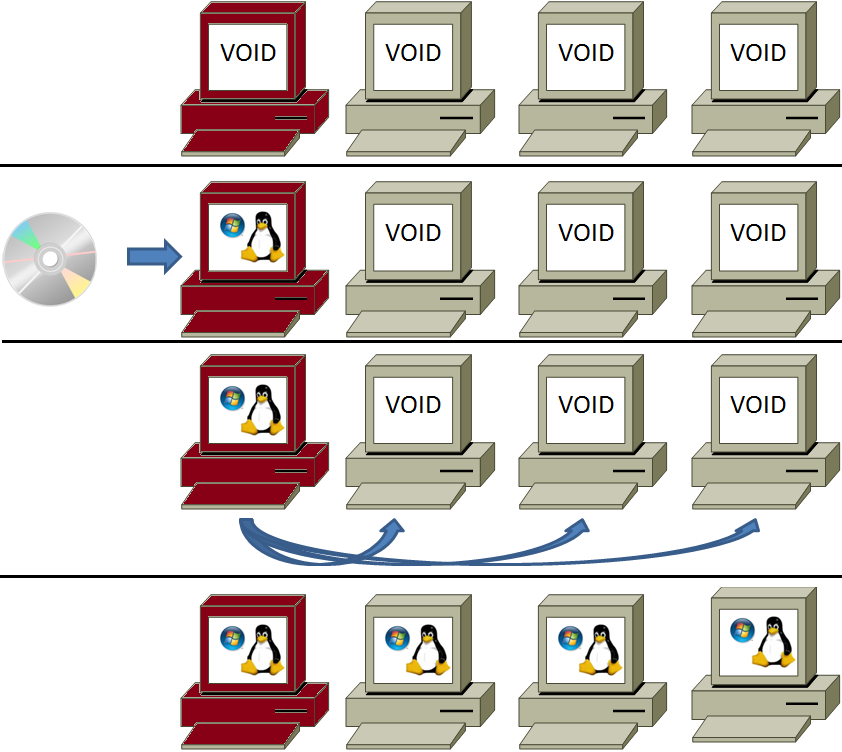
\includegraphics[width=10cm]{img/4comp_seed}
\caption{Seed host (in red)}
\label{fig:s4comp_seed}
\end{figure}

Because of the idea of the seed host being one of the normal hosts in the
network (a decentralised system) certain situations arise where
shortcomings are found. Some of these shortcomings are tried to be resolved
by the subject of this thesis.

\subsection{The Archiving Problem}

After the imaging process, all the hosts should have, at any time, more or
less the same content. The problem is that any old content is lost because
the imaging process means the overwrite of the previous data.

Let us take the example of an University laboratory. Each semester has new
courses with their own labs. Each lab might have different requirements for
the workstations. One lab might use Windows as it's operating system while
the other Linux. One might need an operating system with certain software 
installed while the other other software.

If one laboratory room is used in a year for two courses, one that needs
Setup A and the other Setup B, this means that every semester, an imaging
cycle is needed. This means taking a host, formating it, installing the
required operating system and it's software on it. If Setup A is done at
the beginning of the year, in the second semester, it will be erased and
the next year Setup A will have to be redone.

\subsection{The Backup Problem}

Another situation is where you have a lab with a working operating system
on all computers and a you have a certain lab that specifically asks you to
install an operating system on the host, or modify partitions. This will
cause the radical modification of the hosts and they won't be identical
anymore. Further more some modifications could lead to crashes and render
some hosts useless. The original system would have to be backed up somehow.

One solution is to keep aside one station and after the lab is finished,
use it as a seed to image the other hosts. But this means that you have one
less station to do your lab on.


Another solution is to bring an outside workstation and image it with the
data from the other stations (using one-to-one transfer). This would take
time (because you still need to copy an entire hard disk driver over the
network) and would be logicically hard because you need to bring a station
inside the room and connected with the other ones. Also, the new station
need to have an identical hard drive to receive the data.


\subsection{The Moving Problem}

If you have to image two ore more laboratory rooms (that have the exact
same hardware configuration) with one system image, the two rooms must be
connected to the same network (from a multicast perspective).

If there two rooms are not connected, two things can be done: either do two
separate installs, one in each room, and then run two separate imaging
processes or image in one room and then take one host into the other room
and use it as a seed for the rest of the workstations.

\bigskip

All of the above problems can be resolved by using a centralised system.


\section{The Centralized Approach}

The idea of an imaging system based on UDP Cast is not to rethink what UDP
Cast works or does it's job, but rather to build on top of it and improve
the system and provide and advanced solution for imaging.

The aim of the project is to offer three main features:
\begin{itemize}
\item provide archiving of the system images
\item provide versioning of the system images
\item make a seed server always available and ready to provide images
\end{itemize}

A centralized design requires that a server exists to provide the needed
services. This server will store the system images for all the wanted
setups, each with version history. Clients connect to it and create images
or request archived images. When an images is distributed, the server runs
an udp-sender instance that multicasts the data to the clients.

The server has two main requirements:
\begin{itemize}
\item to be reachable by all the possible clients (eg. all the hosts in all
the laboratory rooms)
\item to have enough storage capacity to hold the images (eg. if you want
to hold up to 3 versions of a system image on a workstation for 40GB of disk
space, you will need at least 120GB of available disk space on the server)
\end{itemize}


\subsection{The Basic Idea}


With this new approach, a new action flow exists, slightly different from
the normal imaging process.


The creation of a system image is still the same. A workstation is cleared
of data, and the needed operating system (or multiple operation systems).
After the setup is done, and the image can be multiplied, the client
program comes in play. Instead of just using the udp-sender to copy data
from the local disk to other disks, it uses a wrapper-client that signals
the Imaging Server that a new image is being created and the Server listens
to a multicast transfer and saves the data locally. The other clients also
receive the image as a normal UDP Cast transfer.


The request for an image is also done via the Client program. One
workstation will have to run the Client to request the image from the
Server. The other clients either start a normal UDP Client, of the Imaging
Clients to receive the image.


To sum up, here are the flow of actions needed:


Image creation:
\begin{itemize}
\item A normal host is prepared with the needed setup. This involves
installing the Operations System(s) and the Software wanted.
\item (Optional) Install the Client locally, as a pseudo operating system,
on a separate partition with a bootloader entry.
\item (Optional) Freeze the system.
\item Launch the Image Client This should be done from a Live Operation
System Environment (or from the locally installed Image Clients as a
separate pseudo operating system, so the installed systems aren't affected.
\item Make a request to the Server to listen for a new image being
transfered.
\item (Optional) Start Image Clients or UDP Cast clients on other
workstations receive the image.
\item Start the transfer.

\end{itemize}
Image request:
\begin{itemize}
\item Start the Image Client on a workstation.
\item Send an Image Request to the Image Server for version of a system
image.
\item Start Clients on the workstations that will be imaged.
\item Start the transfer.
\end{itemize}

\subsection{The Network Boot Server}

The Image Client and the UDP Cast Client should boot from a non-used
operating system, like a Live CD or a network boot. It can either be
installed local as a separate \ac{OS} (different partition) or just as a
separate kernel (using an existing partition) as long as it has a valid
bootloader entry.

Another possibility is to have it as Network Boot Image. This way, as long
as the workstation is connected to the network, it can always boot this
image.

The Network Boot Image requires a PXE Server and the workstations need to
have hardware that supports \ac{PXE} Network Boot. The \ac{DHCP} Server for the local
network need to give out to the hosts the \ac{TFTP} server option so the hosts
can get the image from the \ac{TFTP} Server. The \ac{TFTP} Server will be on the same
machine as the Image Server and have special image with the Image Client.
This image will be a simple linux based distribution.


\section{The Choice of a Framework}

The described architecture can be implemented in verious ways. Some of the
considered were:
\begin{itemize}
\item C and different network libreries
\item Bash and the core-utils programs found in GNU/Linux distributions
\item Python
\item combinations of C, Bash and Python
\end{itemize}

\cite{wiki:python}
Python is a general-purpose high-level programming language whose
design philosophy emphasizes code readability.  Python aims to combine
"remarkable power with very clear syntax",  and its standard library is
large and comprehensive. Its use of indentation  for block delimiters is
unusual among popular programming languages.

Python supports multiple programming paradigms, primarily but not limited
to object oriented, imperative and, to a lesser extent, functional
programming styles. It features a fully dynamic type system and automatic
memory management, similar to that of Scheme, Ruby, Perl, and Tcl. Like
other dynamic languages, Python is often used as a scripting language, but
is also used in a wide range of non-scripting contexts.

The reference implementation of Python (CPython) is free and open source
software and has a community-based development model, as do all or nearly
all of its alternative implementations. CPython is managed by the
non-profit Python Software Foundation.

The choice was Python for 3 main reasons:
\begin{itemize}
\item easier to code compared to C
\item large number of libraries
\item portable to many operating systems
%\item it is open source
\end{itemize}
